\subsection{数据访问对象模式}

数据访问对象模式(Data Access Object pattern)是一种用于抽象数据访问接口的设计模式。它提供了一种方法来访问数据存储,例如关系数据库,而无需关心底层的数据存储技术。

使用数据访问对象模式的主要目的是隔离数据存储和使用层,使两者之间的耦合度降到最低。这样,如果需要更换数据存储技术,只需要修改数据访问对象接口的实现即可,而不需要修改使用数据的代码。

数据访问对象模式通常用于构建大型的,分层的应用程序,例如企业应用程序。在这种应用程序中,数据访问对象模式常常用于把业务逻辑和数据存储分离开来,以便二者可以独立地进行更改和扩展。

总的来说,数据访问对象模式是一种用于提高应用程序的灵活性和可扩展性的设计模式。它可以帮助开发人员更轻松地处理数据存储技术的变化,并使应用程序更容易维护和扩展。

在本项目中,使用数据访问对象模式将单条的traceLog信息进行包装形成TraceLogMO类。设计TraceLogDao接口并配备TraceLogDaoImpl类实现该接口,该类作为数据访问实体类来进行数据访问工作,并在之后供数据传输模块调用。

\begin{figure}[htb]
  \centering
  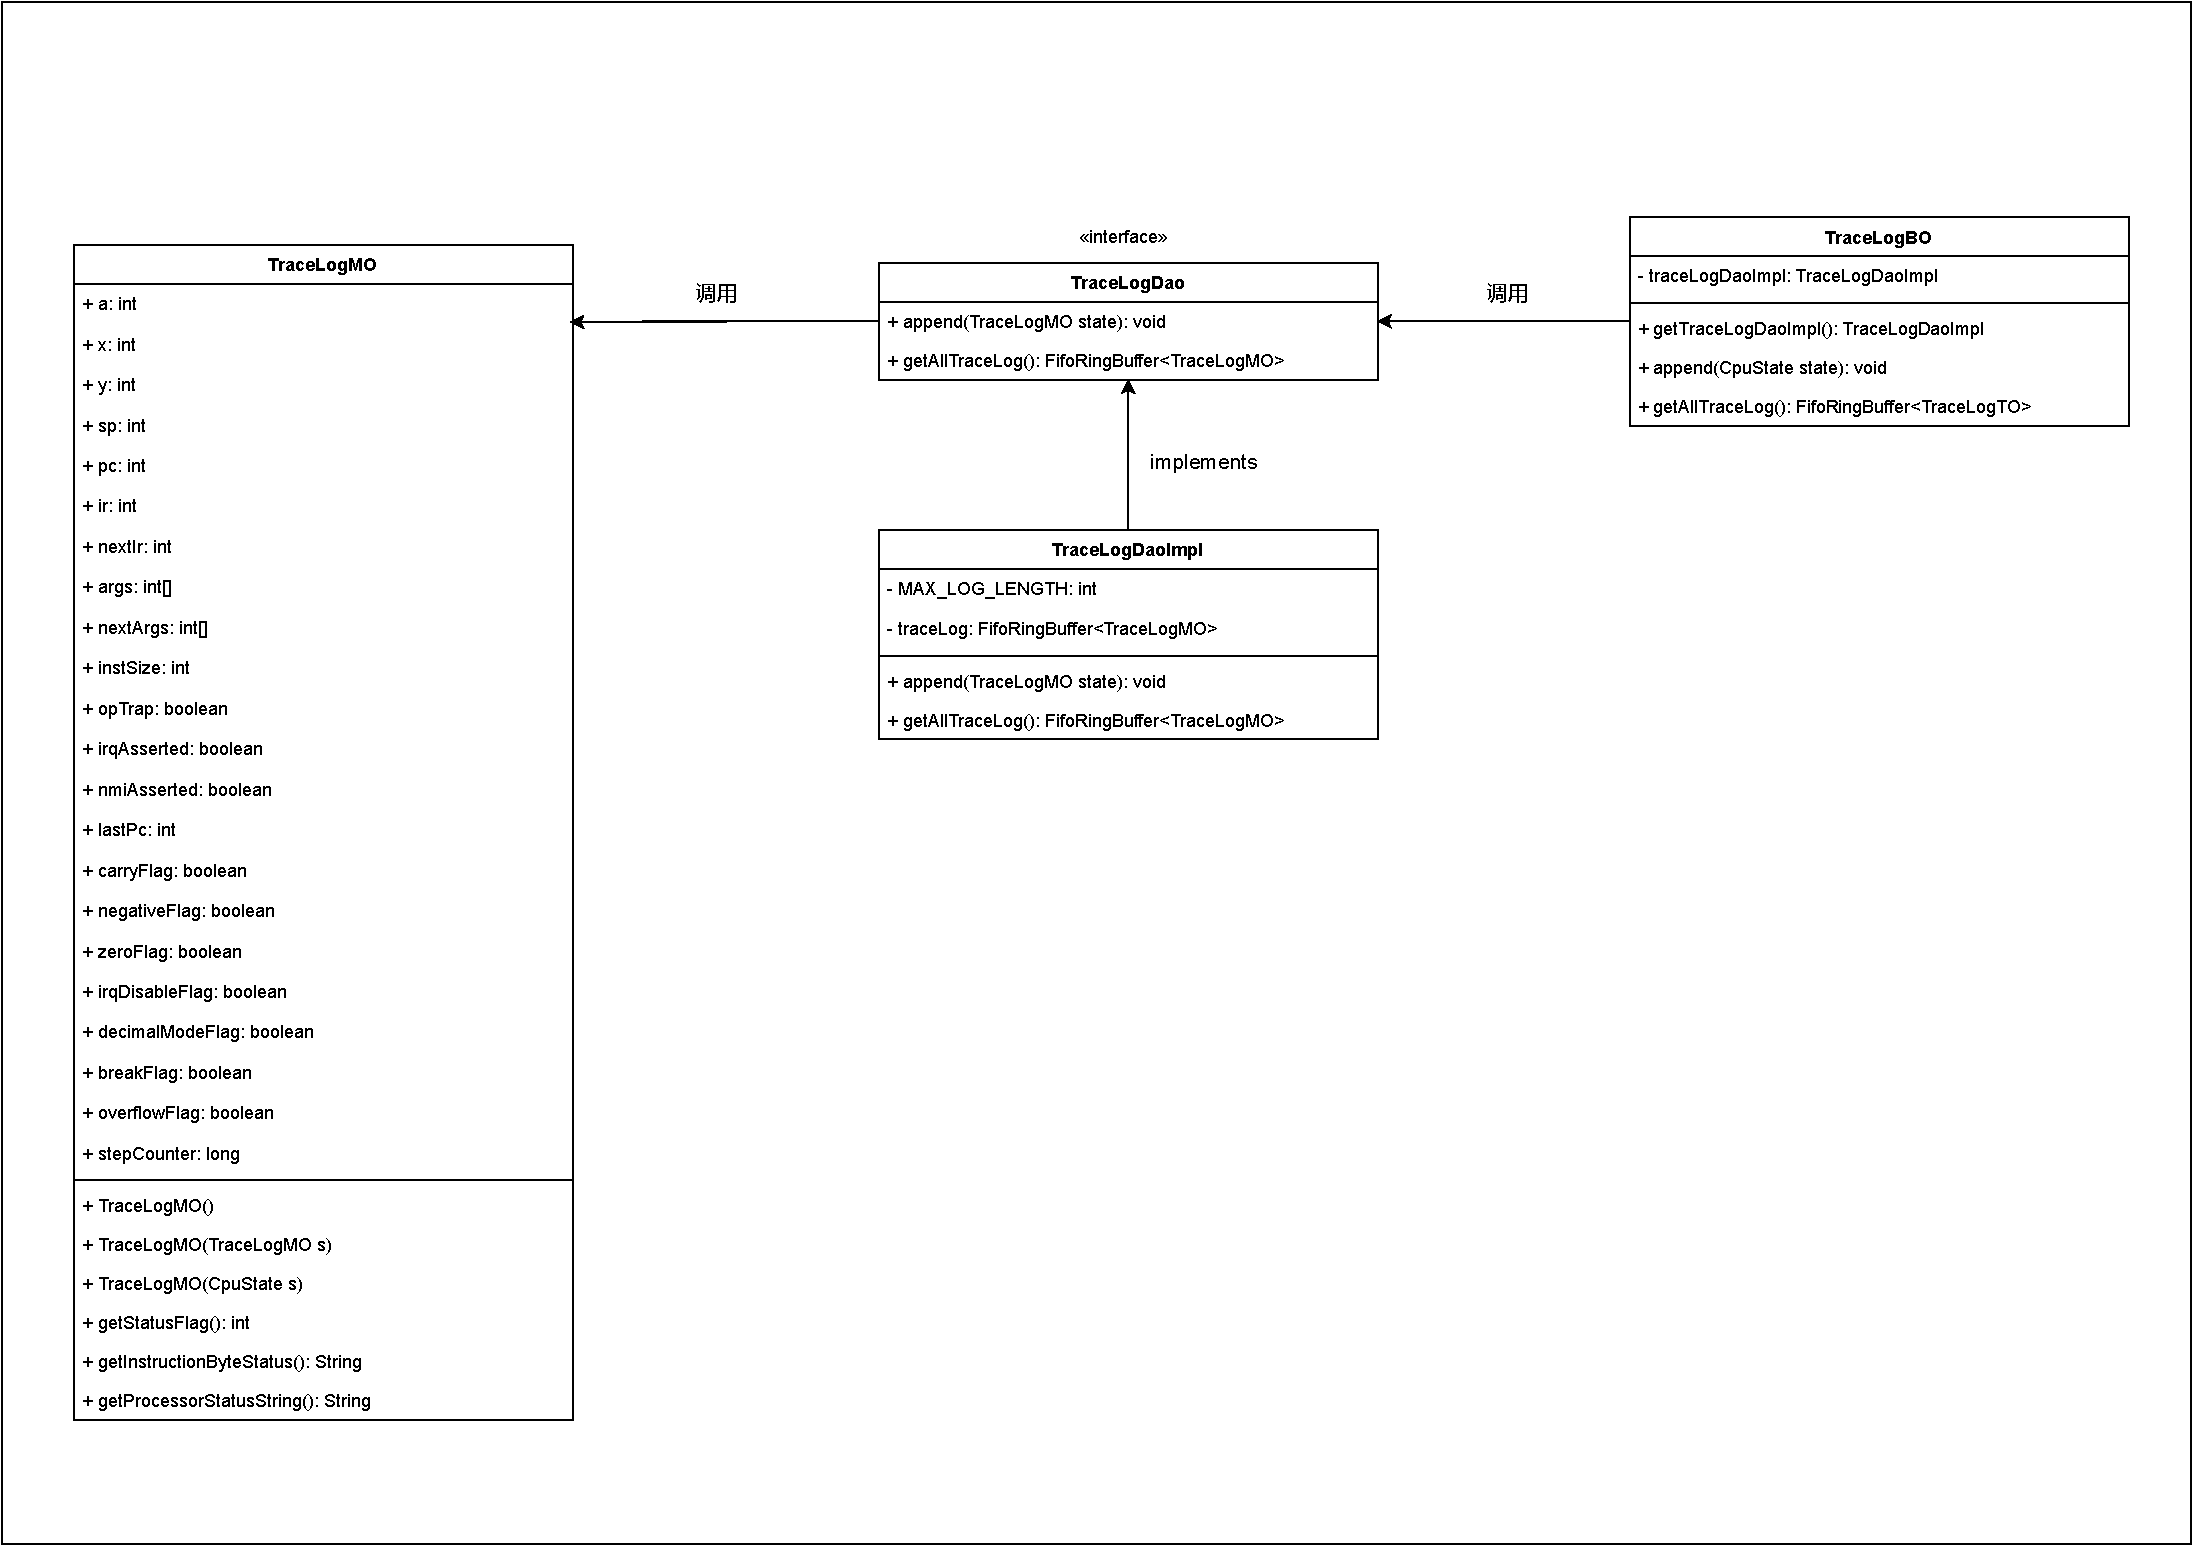
\includegraphics[width=0.9\textwidth]{figures/数据访问对象模式.pdf}
  \caption{数据访问对象模式在 Slow6502 中的类图}
\end{figure}
